\section{Clase 6 - Pr\'actica 3 (Ecuaciones diferenciales - Problema de valores de contorno)}

\underline{Definici\'on 1}: Decimos que el m\'etodo es consistente si $T \rightarrow_{h \rightarrow 0,\ k \rightarrow 0} 0$.\\

\underline{Definici\'on 2}: Decimos que el m\'etodo es estable en norma $\|.\|$ si existe una constante $C > 0$ (independiente de $h, k, j, n, J, N$) tal que $\|u^{n}\| \leq C\|u^{0}\|$.\\

Veamos cuando este m\'etodo es estable en norma $\infty$, $\|v\|_{\infty} = \max \limits_{j} \{|v_{j}|\}$.

$$\|u^{n + 1}\|_{\infty} = \max \limits_{j} \bigg\{\bigg| \frac{k}{h^{2}}u_{j - 1}^{n} + \bigg(1 - \frac{2k}{h^{2}}u_{j}^{n}\bigg) +  \frac{k}{h^{2}}u_{j + 1}^{n} \bigg| \bigg\} \leq \max \limits_{j} \bigg\{\bigg| \frac{k}{h^{2}}\|u_{j - 1}^{n}\|_{\infty} + \bigg|1 - \frac{2k}{h^{2}}\bigg|\|u_{j}^{n}\|_{\infty} +  \frac{k}{h^{2}}\|u_{j + 1}^{n}\|_{\infty} \bigg\}$$

$$\Rightarrow \|u^{n + 1}\|_{\infty} \leq \bigg(\frac{2k}{h^{2}} +   \bigg|1 - \frac{2k}{h^{2}}\bigg|\bigg)\|u^{n}\|_{\infty}$$

Si $\frac{2k}{h^{2}} < 1$, o sea, $2k < h^{2},\ \|u^{n + 1}\|_{\infty} \leq \|u^{n}\|_{\infty}$. Con este razonamiento concluimos $\|u^{n + 1}\|_{\infty} \leq \|u^{0}\|_{\infty}$ y el m\'etodo resulta estable con $C = 1$.\\

\underline{Error}:

$$u(x_{j}, t_{n + 1}) = \frac{k}{h^{2}}u(x_{j - 1}, t_{n}) + \bigg(1 - \frac{2k}{h^{2}}\bigg)u(x_{j}, t_{n}) + \frac{k}{h^{2}}u(x_{j - 1}, t_{n})+ k\tau_{j}^{n}$$

$$u_{j}^{n + 1} = \frac{k}{h^{2}}u_{j - 1}^{n} + \bigg(1 - \frac{2k}{h^{2}}\bigg)u_{j}^{n} + \frac{k}{h^{2}}u_{j + 1}^{n}$$

$$\Rightarrow e_{j}^{n + 1} = u(x_{j}, t_{n + 1}) - u_{j}^{n + 1} = \frac{k}{h^{2}}e_{j - 1}^{n} + \bigg(1 - \frac{2k}{h^{2}}\bigg)e_{j}^{n} + \frac{k}{h^{2}}e_{j + 1}^{n} + k\tau_{j}^{n}$$

\underline{Definici\'on 3}: Decimos que el m\'etodo es convergente si $\max \limits_{j, n} e_{j}^{n} \rightarrow_{h \rightarrow 0,\ k \rightarrow 0} 0$.\\

Llamamos $e^{n} = \max \limits_{j} \{|e_{j}^{n}|\}$ y $\tau^{n} = \max \limits_{j} \{|\tau_{j}^{n}|\}$, entonces

$$|e_{j}^{n + 1}| \leq \frac{k}{h^{2}}|e_{j - 1}^{n}| + \bigg|1 - \frac{2k}{h^{2}}\bigg||e_{j}^{n}| + \frac{k}{h^{2}}|e_{j}^{n}| + k|\tau_{j}^{n}|$$

$$|e_{j}^{n + 1}| \leq \frac{k}{h^{2}}e^{n} + \bigg|1 - \frac{2k}{h^{2}}\bigg|e^{n} + \frac{k}{h^{2}}e^{n} + k\tau^{n}$$

$$|e_{j}^{n + 1}| \leq e^{n} + k\tau^{n}$$

$$e^{n + 1} \leq e^{n} + k\tau^{n} \leq e^{0} + (k\tau^{0} + \cdots + k\tau^{n}) \leq (k\tau^{0} + \cdots + k\tau^{n}) = k \sum \limits_{i = 0}^{n} \tau^{i} \leq k(n + 1) \max \limits_{i} \max \limits_{j} |\tau_{i}^{j}|,\ n \leq N - 1$$

$$\Rightarrow e^{n + 1} \leq k(n + 1)[\mathcal{O}(k) + \mathcal{O}(h^{2})] \leq kN[\mathcal{O}(k) + \mathcal{O}(h^{2})] = T_{F}[\mathcal{O}(k) + \mathcal{O}(h^{2})],\ k = \frac{T_{F}}{N}$$

y el m\'etodo resulta convergente cuando $h \rightarrow 0,\ k \rightarrow 0$.\\

\begin{itemize}
	\item Notemos que si $h = 10^{-3}$, estamos pidiendo $2k < 10^{-6}$, es decir, $2\cdot10^{6} < N$.
\end{itemize}

Veamos un m\'etodo impl\'icito

$$ 
	\begin{cases}
		\frac{u_{j}^{n + 1} - u_{j}^{n}}{k} = \frac{u_{j + 1}^{n} - 2u_{j}^{n} + u_{j - 1}^{n}}{h^{2}},\ 1 \leq j \leq J - 1,\ 1 \leq n \leq N - 1\\
		u_{j}^{0} = g(x_{j}),\ 0 \leq j \leq J\\
		u_{0}^{n} = u_{J}^{n},\ 0 \leq n \leq N\\
    \end{cases}
$$

Despejamos: 

$$u_{j}^{n + 1} = -\frac{k}{h^{2}}u_{j - 1}^{n} + \bigg(1 + \frac{2k}{h^{2}}\bigg)u_{j}^{n} - \frac{k}{h^{2}}u_{j + 1}^{n}$$

Forma matricial:

$$
	\begin{pmatrix}
        u_{1}^{n + 1}\\
        \vdots\\
        \vdots\\
        u_{J - 1}^{n + 1}\\
	\end{pmatrix}
	=
    \begin{pmatrix}
        1 + \frac{2k}{h^{2}} & -\frac{k}{h^{2}} & \cdots\\
        -\frac{k}{h^{2}} & \cdots & \cdots\\
        \vdots & \vdots & \vdots\\
        \cdots & \cdots & \cdots\\

	\end{pmatrix}
    \begin{pmatrix}
        u_{1}^{n}\\
        \vdots\\
        \vdots\\
        u_{J - 1}^{n}\\
	\end{pmatrix}
$$

y debemos resolver el sistema lineal $A^{-1}u^{n} = u^{n + 1}$.\\

Verificar que vale:

\begin{itemize}
	\item $\tau = \mathcal{O}(k) + \mathcal{O}(h^{2})$

	\item $\bigg(1 + \frac{2k}{h^{2}}\bigg)e_{j}^{n + 1} = e_{j}^{n} + \frac{k}{h^{2}}e_{j - 1}^{n + 1} + \frac{k}{h^{2}}e_{j + 1}^{n + 1} + k\tau_{j}^{n + 1}$
\end{itemize}

Luego,

$$\bigg(1 + \frac{2k}{h^{2}}\bigg)|e_{j}^{n + 1}| \leq |e_{j}^{n}| + \frac{k}{h^{2}}|e_{j - 1}^{n + 1}| + \frac{k}{h^{2}}|e_{j + 1}^{n + 1}| + k|\tau_{j}^{n + 1}| \leq e^{n} + \frac{k}{h^{2}}e^{n + 1} + \frac{k}{h^{2}}e^{n + 1} + k\tau^{n + 1}$$

$$\Rightarrow e^{n + 1} \leq e^{n} + k\tau^{n + 1} \leq e^{n - 1} + k\tau^{n} + k\tau^{n + 1} \leq e^{0} + k(\tau^{1} + \cdots + \tau^{n + 1}) \leq k \sum \limits_{j = 1}^{n} \tau^{j} \leq k(n + 1) \max \limits_{i} \max \limits_{j} |\tau_{i}^{j}|$$

$$\Rightarrow e^{n + 1} \leq T_{F}[\mathcal{O}(k) + \mathcal{O}(h^{2})],\ n \leq N - 1$$

Cu\'al es la diferencia con el m\'etodo expl\'icito? En el m\'etodo impl\'icito NO necesitamos la condici\'on $2k < h^{2}$.\\

\textit{Python}: Diferencias finitas. Ecuaci\'on del calor

$$ 
	\begin{cases}
        u_{t}(x, t) = \alpha u_{xx}(x, t),\ x \in (0, 1)\\
        u(x, 0) = g(x) = \sin(\pi x),\ t \in [0, 1]\\
        u(0, t) = u(1, t) = 0,\ t > 0\\
    \end{cases}
$$

\begin{verbatim}
	import numpy as np
	import matplotlib.pyplot as plt
	
	def g(x):
	    return np.sin(np.pi * x)
		
	def DifFinitasCalor(x0, xf, t0, tf, alpha, DeltaX, DeltaT, g):
	    N = int((xf - x0) / DeltaX)
	    x = np.linspace(x0, xf, N + 1)
	    M = int((tf - t0) / DeltaT)
	    t = np.linspace(t0, tf, N + 1)
	    
	    u = np.zeros((M + 1, N + 1))
	    
	    u[0, :] = g(x)
	    
	    r = DeltaT / (DeltaX**2)
		
	    Diag = np.ones(N - 1) * (1 - 2 * alpha * r)
	    DiagArriba = np.ones(N - 2) * (alpha * r)
	    
	    A = np.diag(Diag) + np.diag(DiagArriba, 1) + np.diag(DiagArriba, -1)
	    
	    for i in range(1, M + 1):
	        u[i, 1:N] = A@u[i - 1, 1:N]
	    
	    return (t, u)
		
	x0 = 0
	xf = 1
	t0 = 0
	tf = 10
	alpha = 1
	DeltaX = 0.1
	DeltaT = 0.001
	
	t, u = DifFinitasCalor(x0, xf, t0, tf, alpha, DeltaX, DeltaT, g)
	
	print(t)
	print(u)
	
	M = int((tf - t0) / DeltaT)
	N = int((xf - x0) / DeltaX)
	
	x = np.linspace(x0, xf, N + 1)
	
	for i in range(0, M):
	    plt.plot(x, u[i, :])
\end{verbatim}

\begin{figure}[H]
  \centering
  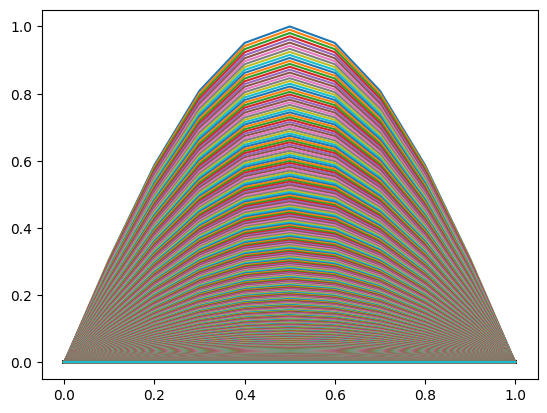
\includegraphics[width=0.6\linewidth]{Clase6_Practica3/difs_c6p3.png}
\end{figure}